\begin{figure*}[p]
\section*{E. Harness Architectures and Implementation Details}
\label{app:artifact-details}
\subsection*{E.1 ALFWorld}
\centering
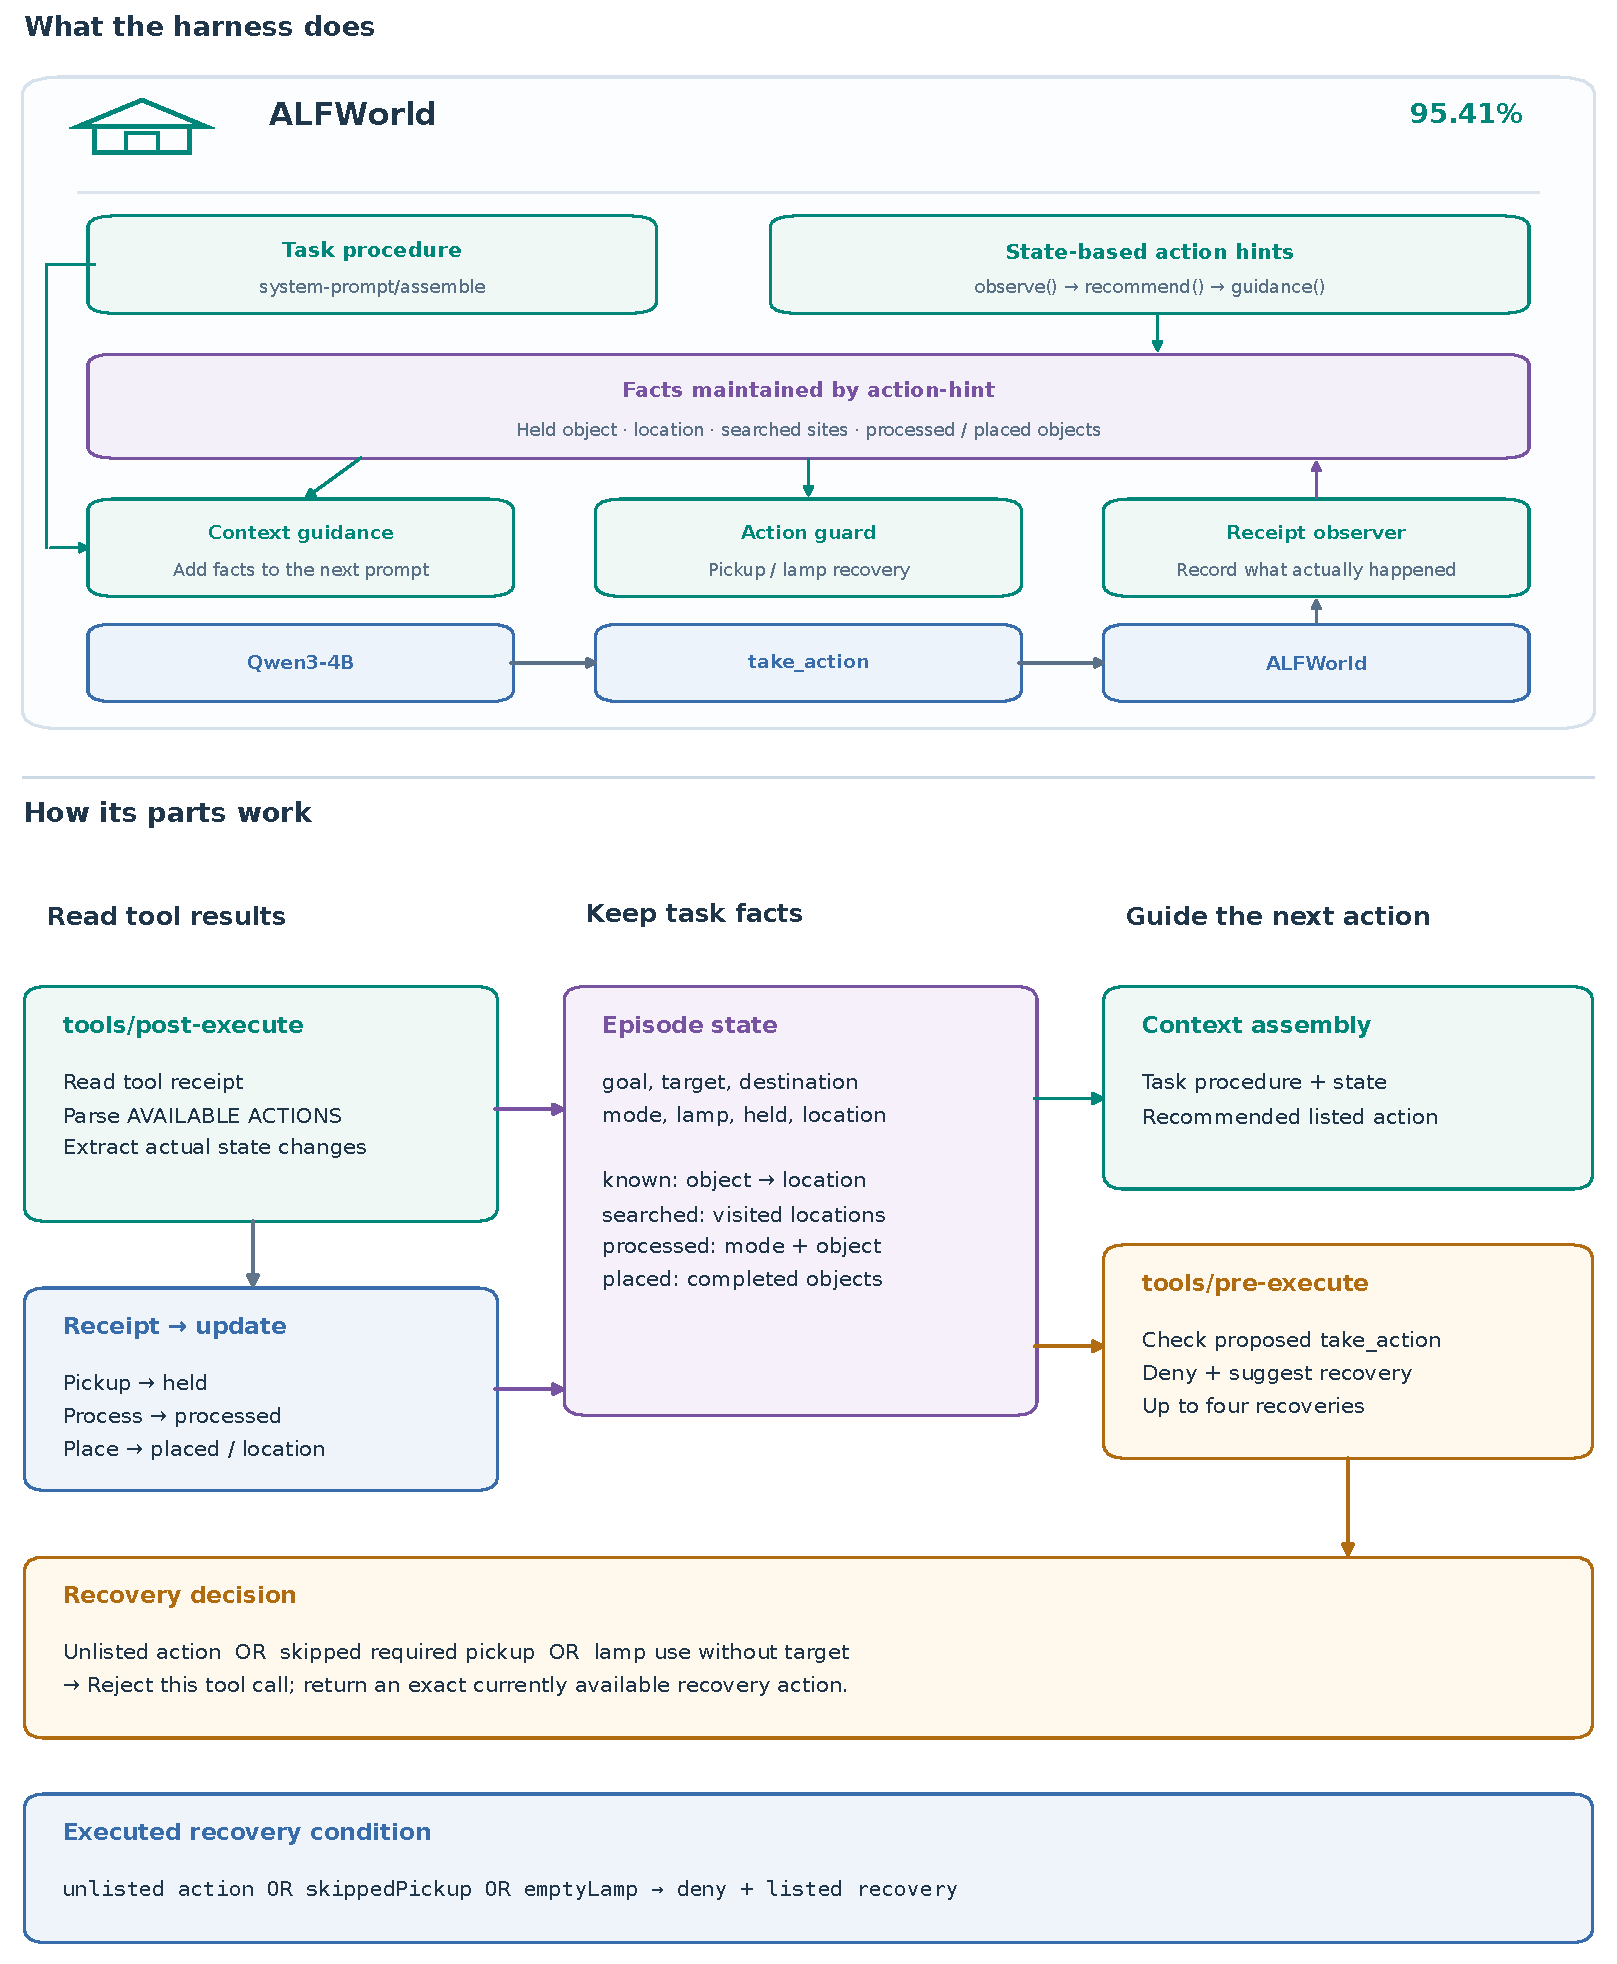
\includegraphics[width=\textwidth,height=.80\textheight,keepaspectratio]{dsh-draft/figures/harness-artifacts/alfworld-architecture.pdf}
\caption{Architecture and implementation details of ALFWorld v06. The overview names component responsibilities; the lower panels expand the corresponding source modules and state updates. The action-hint plugin parses actual receipts into task-local state, uses that state for context guidance, and checks proposed actions before execution. Recovery is bounded to four interventions per task. The task-guide plugin supplies the household procedure.}
\label{fig:artifact-alfworld-detail}
\end{figure*}
\begin{figure*}[p]
\subsection*{E.2 DBBench}
\centering
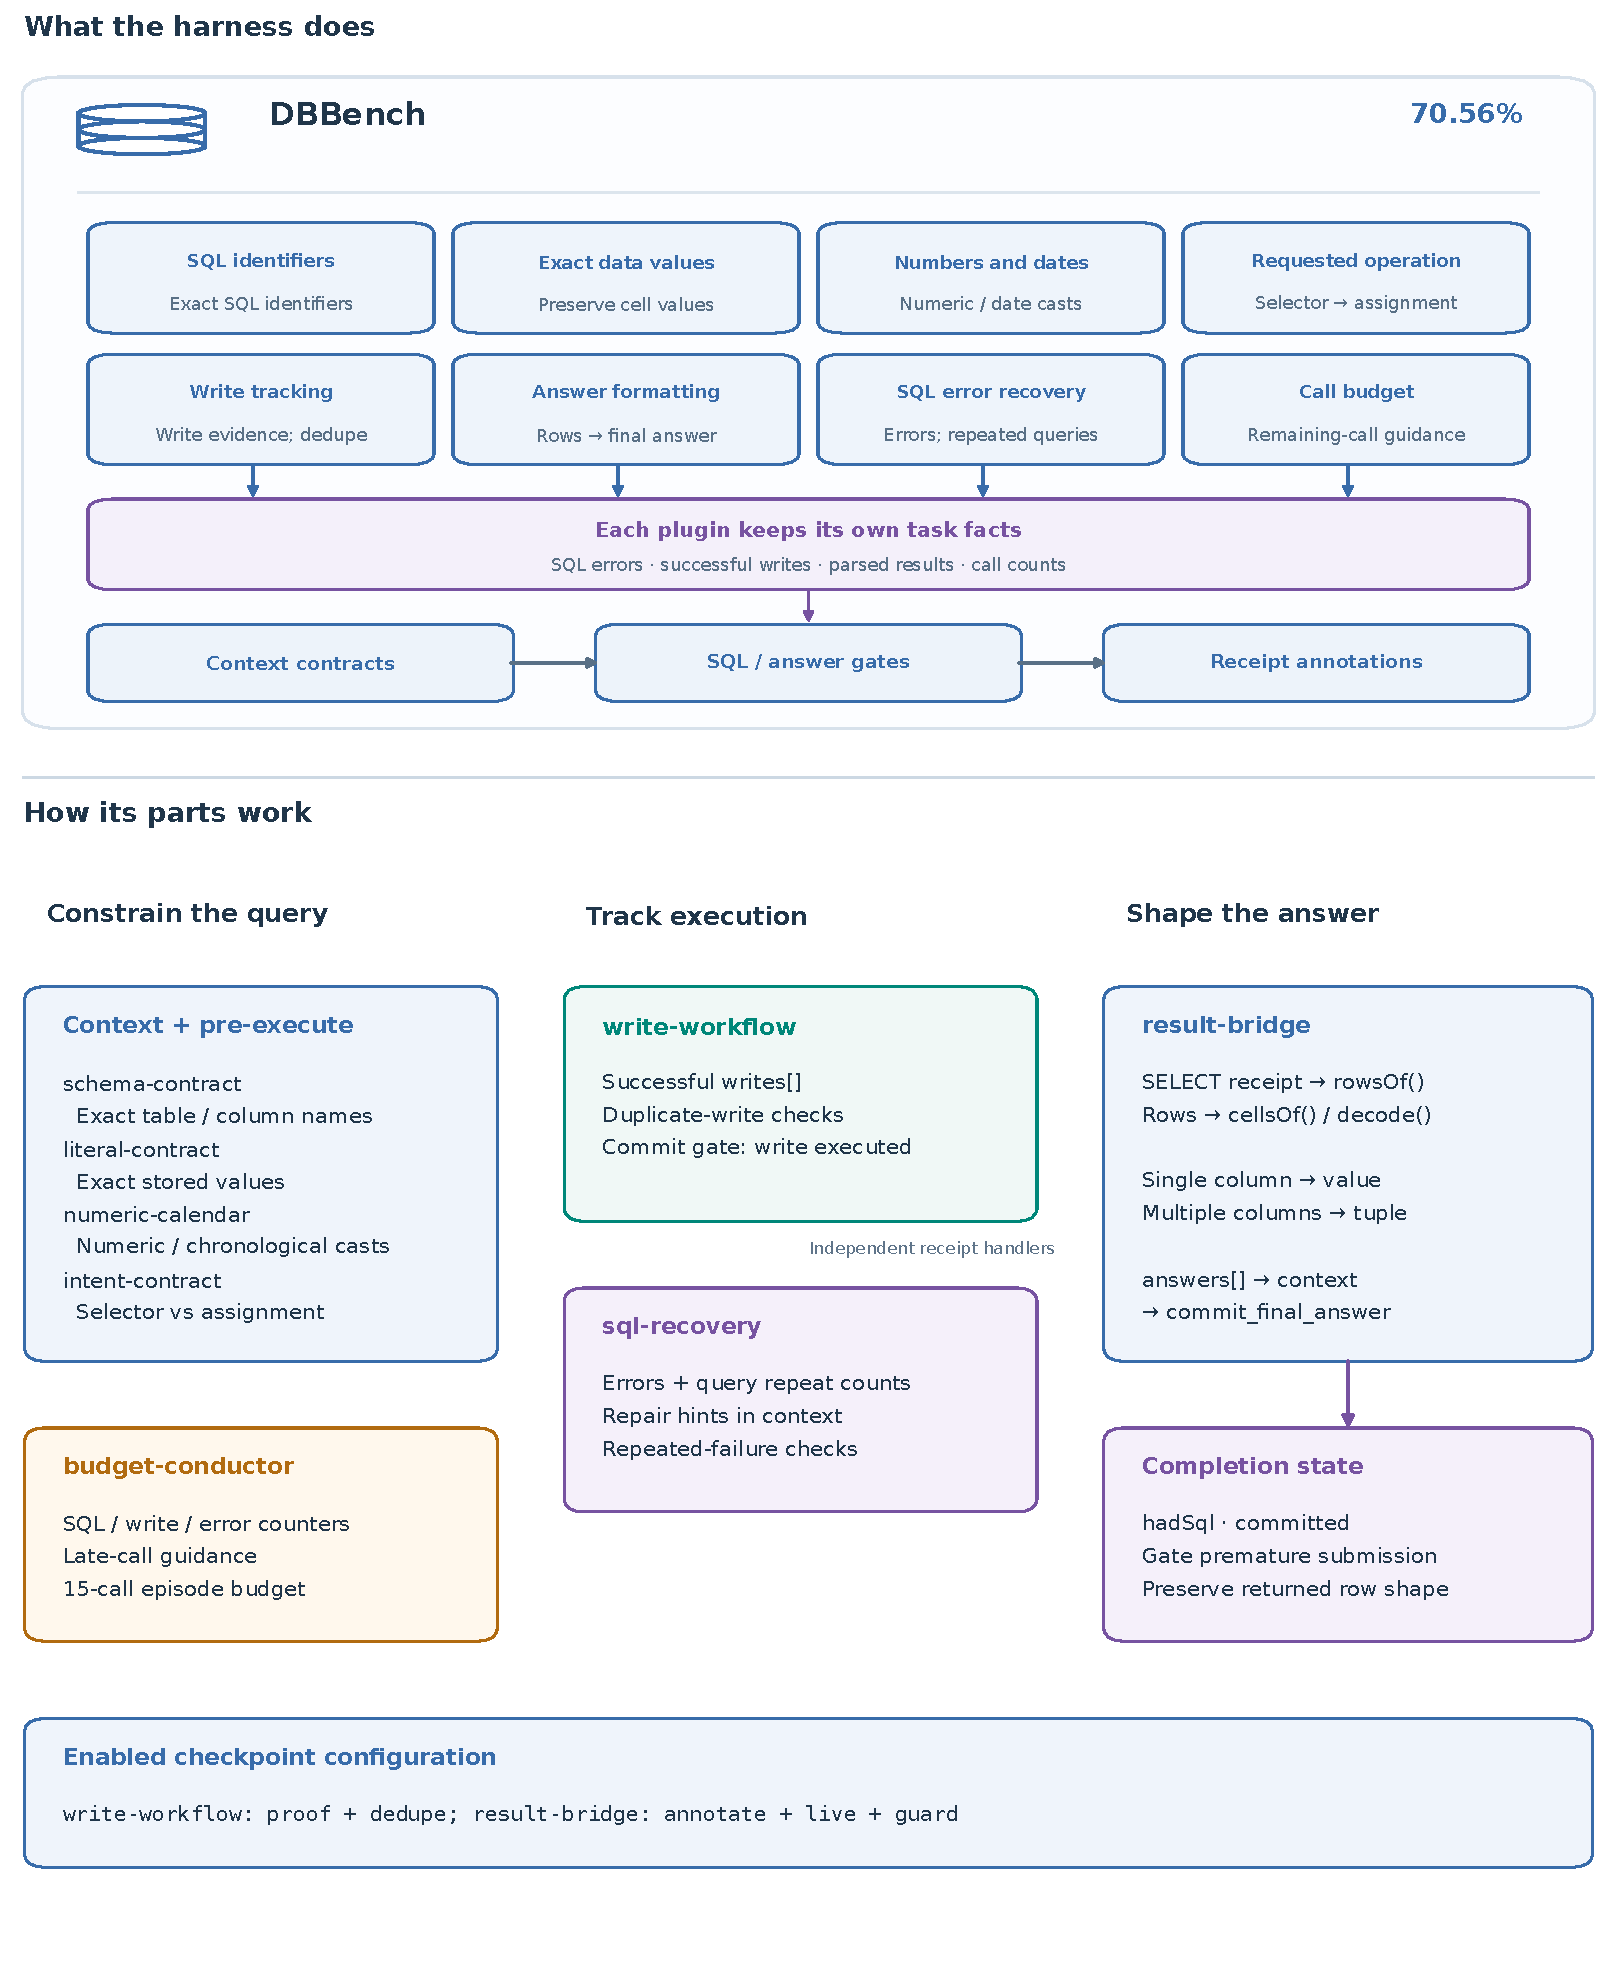
\includegraphics[width=\textwidth,height=.80\textheight,keepaspectratio]{dsh-draft/figures/harness-artifacts/dbbench-architecture.pdf}
\caption{Architecture and implementation details of DBBench v35. Context contracts constrain SQL construction; write-workflow, sql-recovery, and budget-conductor maintain their own execution records. The result-bridge parses returned rows into native final-answer arguments. Arrows summarize the execution and information-processing stages; plugin states remain local.}
\label{fig:artifact-dbbench-detail}
\end{figure*}
\begin{figure*}[p]
\subsection*{E.3 WebShop}
\centering
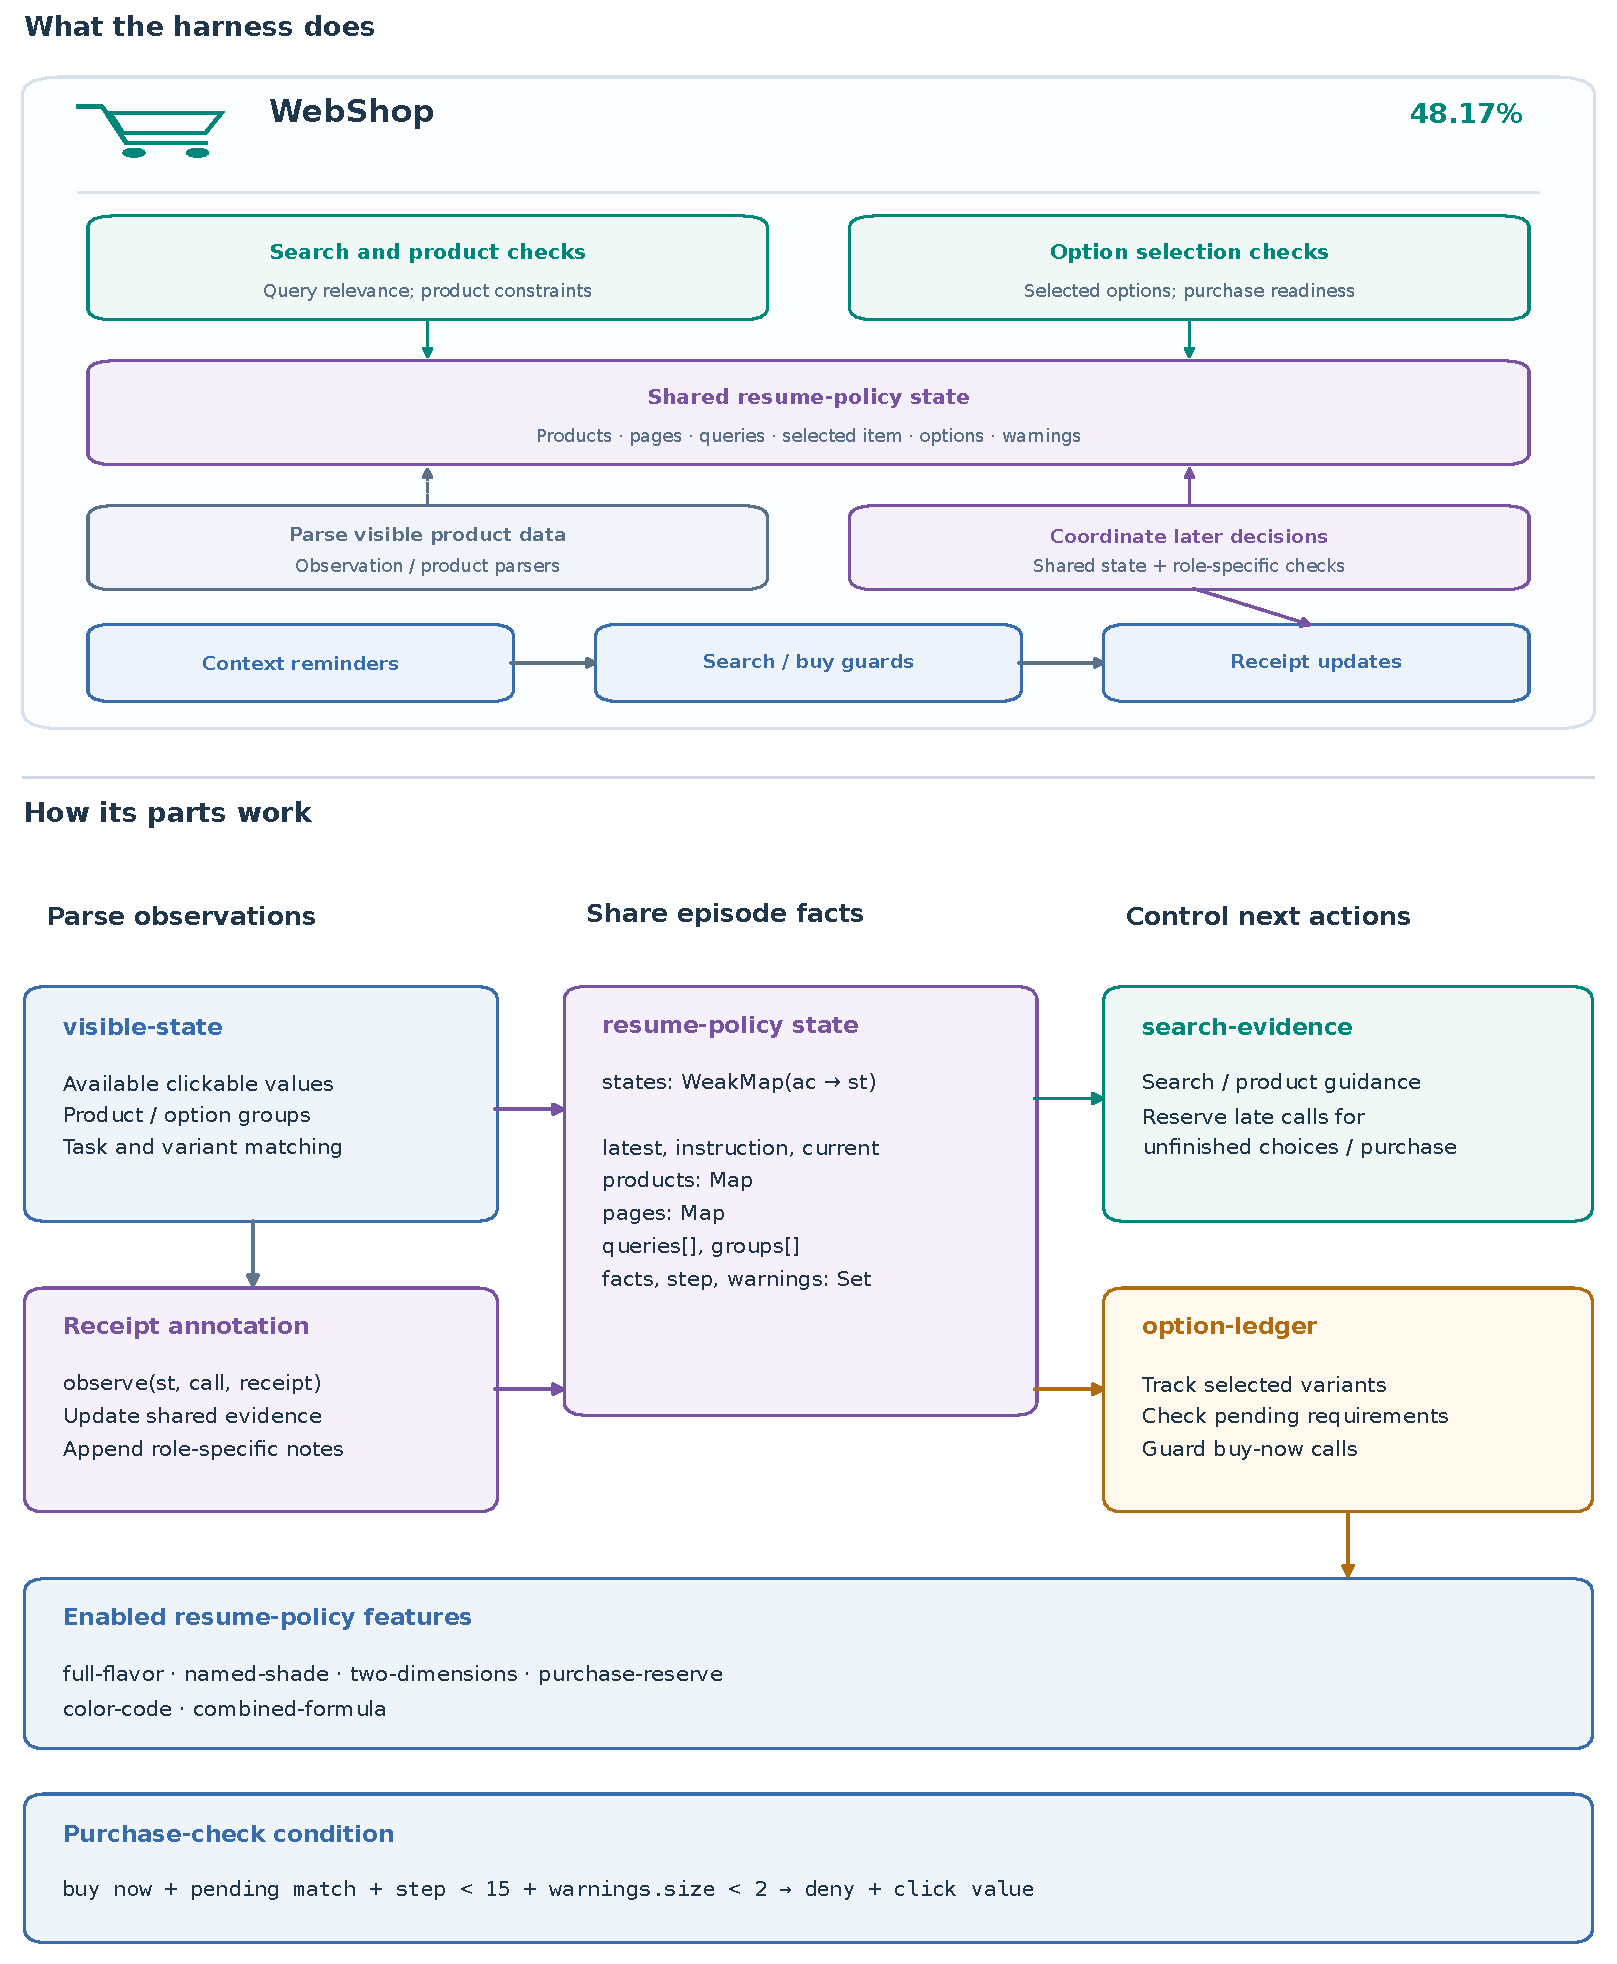
\includegraphics[width=\textwidth,height=.80\textheight,keepaspectratio]{dsh-draft/figures/harness-artifacts/webshop-architecture.pdf}
\caption{Architecture and implementation details of WebShop continuation v12. Both enabled plugin roles import visible-state utilities and install resume-policy handlers. The latter share state through an agent-keyed WeakMap. Receipt observations update the facts used for subsequent search and purchase checks. The bottom path summarizes a condition implemented by the option-ledger role.}
\label{fig:artifact-webshop-detail}
\end{figure*}
\begin{figure*}[p]
\subsection*{E.4 OSBench}
\centering
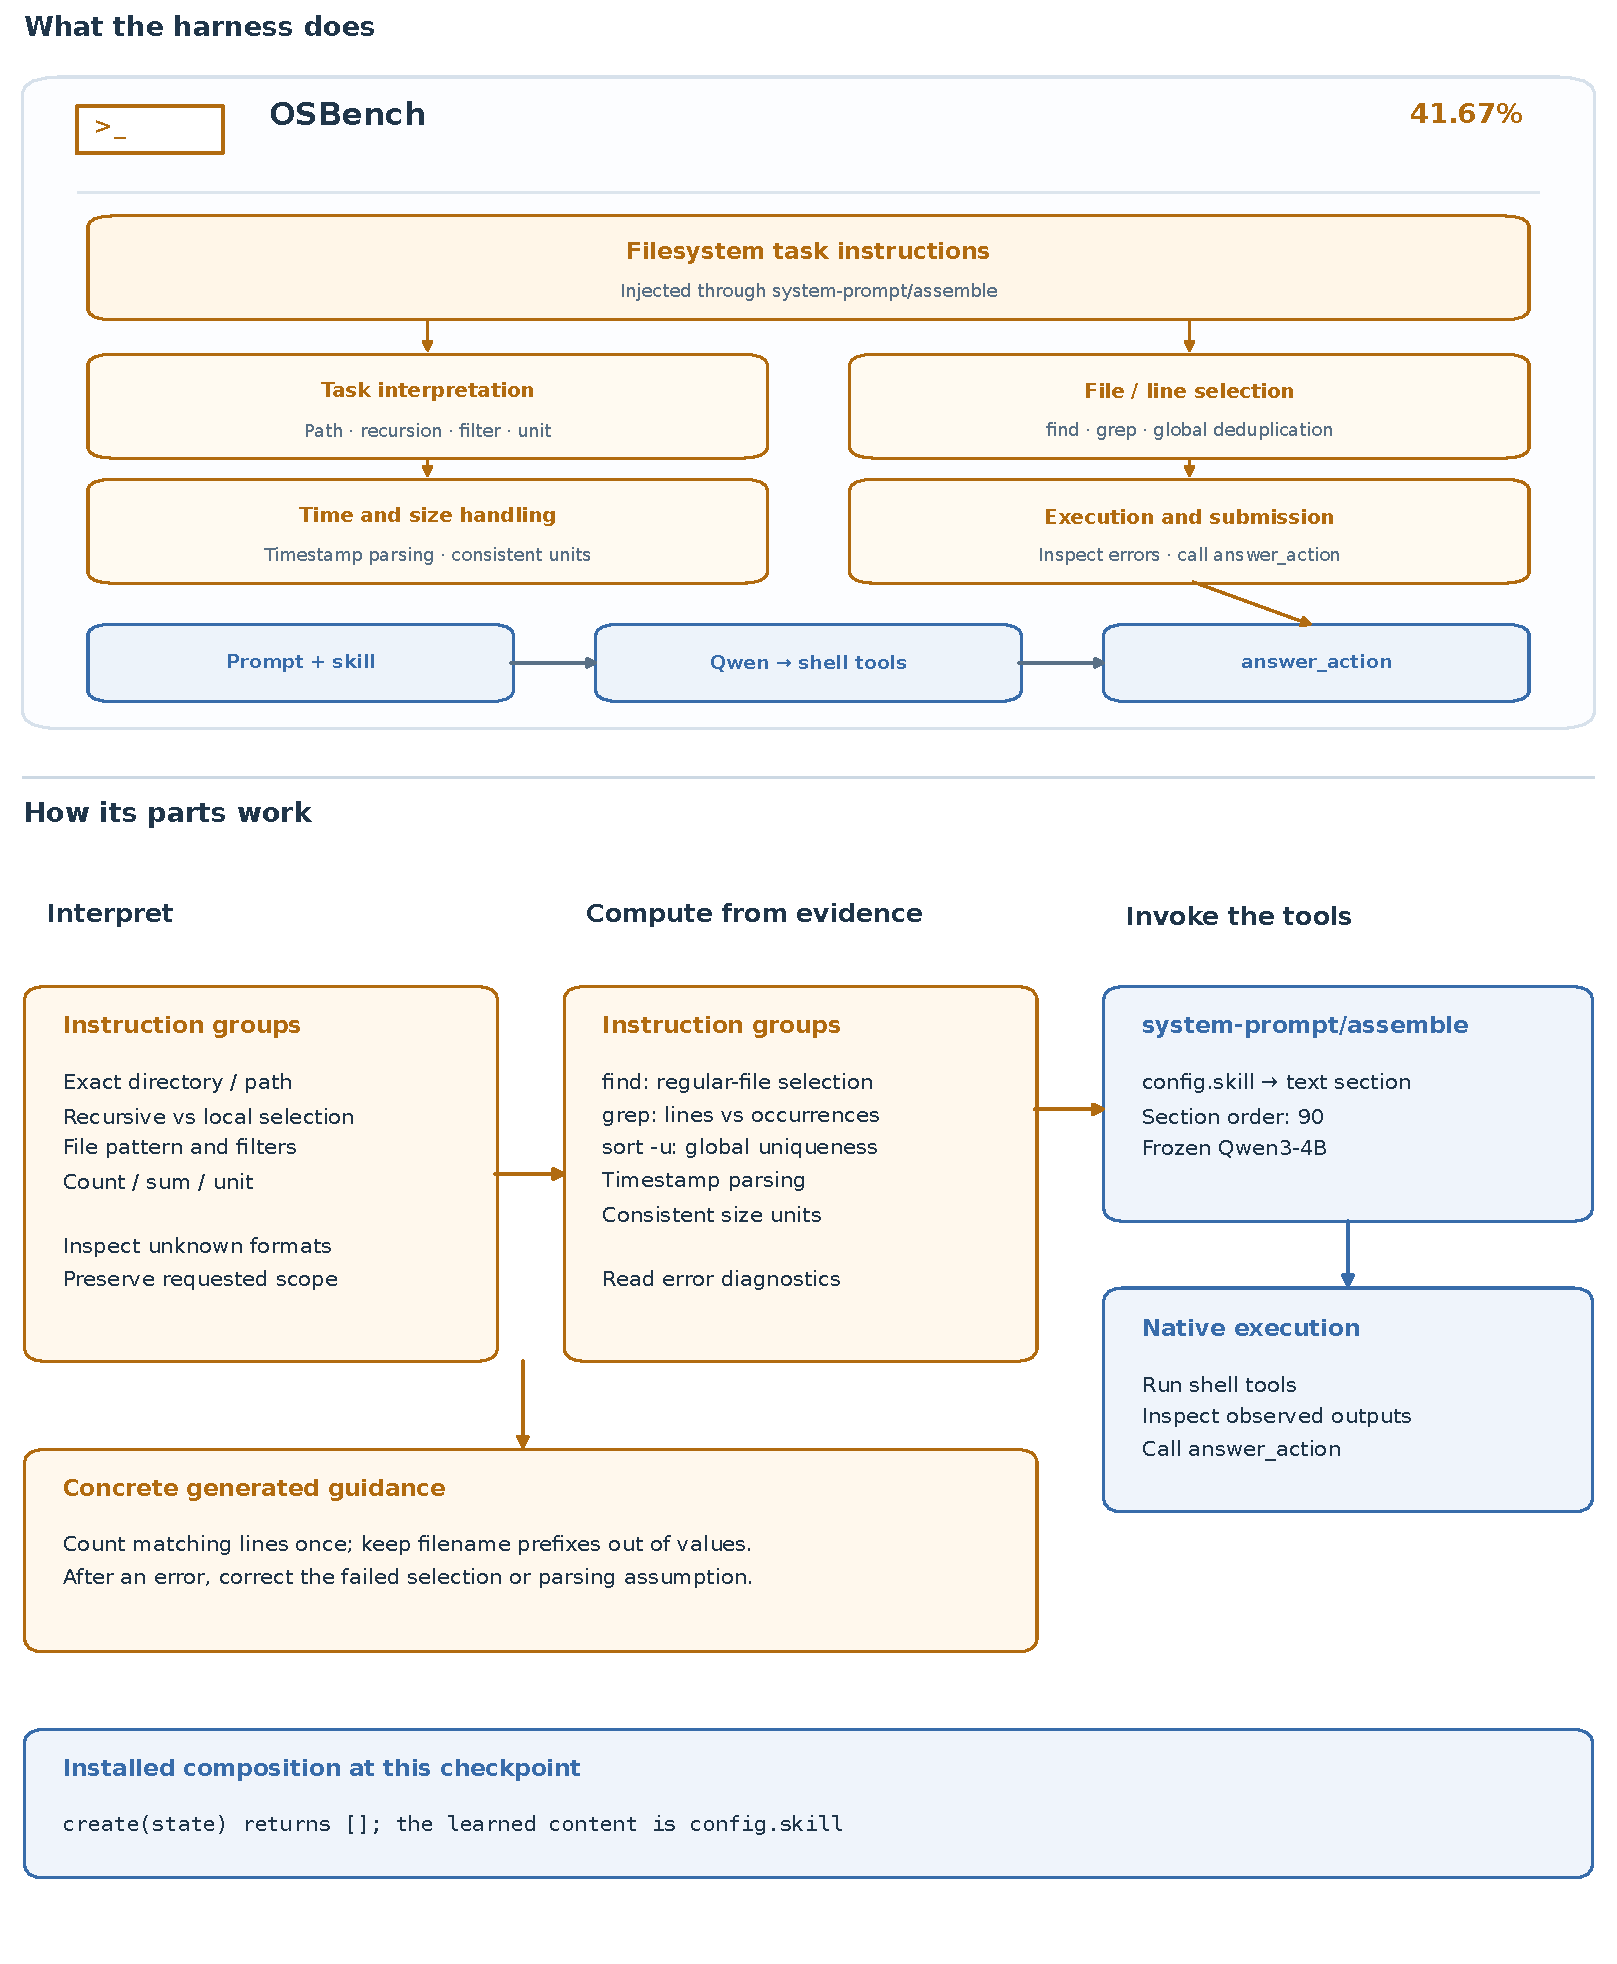
\includegraphics[width=\textwidth,height=.80\textheight,keepaspectratio]{dsh-draft/figures/harness-artifacts/osbench-architecture.pdf}
\caption{Architecture and implementation details of OSBench v01. The retained artifact is the skill text supplied through scale-slot. The orange groups expand its instructions for selecting files, counting and aggregating evidence, handling dates and units, and submitting through the native tool. They are instruction groups rather than separately generated executable modules.}
\label{fig:artifact-osbench-detail}
\end{figure*}
